\begin{example}~
\label{ex:two_channels}
	Suppose we have the set of confidential information represented as $P = \set{(1,3),(2,1),(3,4),(4,1),(5,5),(6,9)}$. Suppose that \AgentOne sends this information encrypted as $Q = \set{(1,12),(2,1),(3,16),(4,1),(5,17),(6,18)}$. In order to further conceal the information, \AgentOne decides to send the information at odd times on one channel and the information at even times on a second channel such that $Q_1 = \set{(1,12),(3,16),(5,17)}$ and $Q_2 = \set{(2,1),(4,1),(6,18)}$. \newline 

	We define the relations $P$, $Q_1$ and $Q_2$ in \relview\ as follows: \newline

	\begin{figure}[ht]
		\centering
		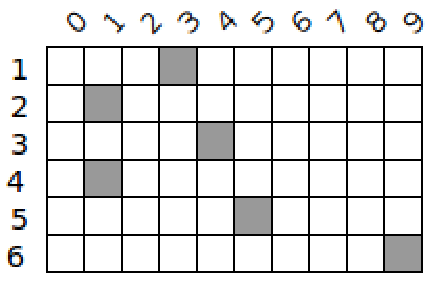
\includegraphics[scale=0.65]{Figures/PDF/Relview/P.pdf}
		\caption{Relation $P$ for Example~\ref{ex:two_channels}.}
		\label{fig:two_channels_p}
	\end{figure}
	
	\begin{figure}[ht]
		\centering
		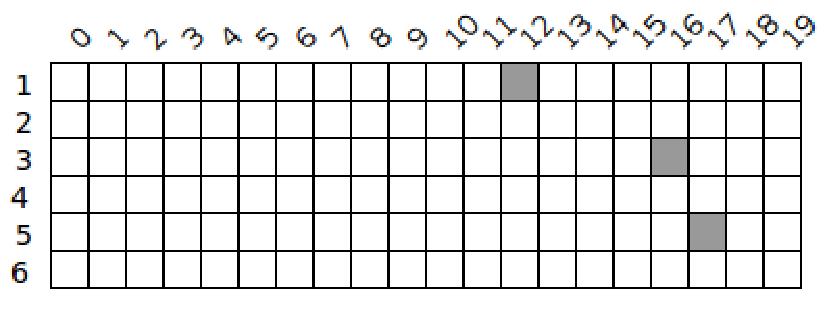
\includegraphics[scale=0.65]{Figures/PDF/Relview/Q1.pdf}
		\caption{Relation $Q_1$ for Example~\ref{ex:two_channels}.}
		\label{fig:two_channels_q1}
	\end{figure}

	\begin{figure}[ht]
		\centering
		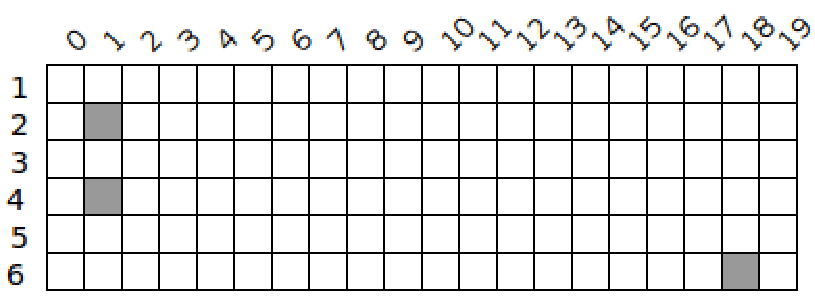
\includegraphics[scale=0.65]{Figures/PDF/Relview/Q2.pdf}
		\caption{Relation $Q_2$ for Example~\ref{ex:two_channels}.}
		\label{fig:two_channels_q2}
	\end{figure}
	
	\newpage
	Assume that the analyst has programmed the monitor of the communication channels to combine the information that has been sent on the channels corresponding to $Q_1$ and $Q_2$ with the union operation ( $\!\!\!\STjoin\!\!\!$ ). Then, we verify the existence of an abstraction relation by executing Program~\ref{prog:test} ($Result = Test(P, (Q_1 \STjoin Q_2))$). \newline
	
	\begin{figure}[ht]
		\centering
		
\includegraphics[scale=0.65]{Figures/PDF/Relview/True.pdf}
		\caption{Relation $Result$ for Example~\ref{ex:two_channels}.}
		\label{fig:two_channels_result}
	\end{figure}

	Therefore, the test has passed meaning that an abstraction relation relating the confidential information to the information observed to be sent on the communication channels. We run Program~\ref{prog:compute} ($X = Compute(P,(Q_1 \STjoin Q_2),R)$) to obtain the abstraction relation where $R$ is the filtering relation. \newline

	\begin{figure}[ht]
		\centering
		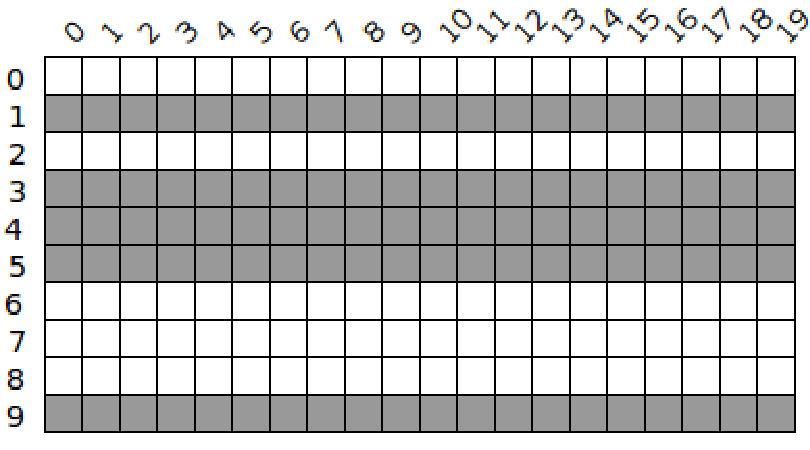
\includegraphics[scale=0.65]{Figures/PDF/Relview/R.pdf}
		\caption{Filtering relation $R$ for Example~\ref{ex:two_channels}.}
		\label{fig:two_channels_r}
	\end{figure}
	
	\begin{figure}[ht]
		\centering
		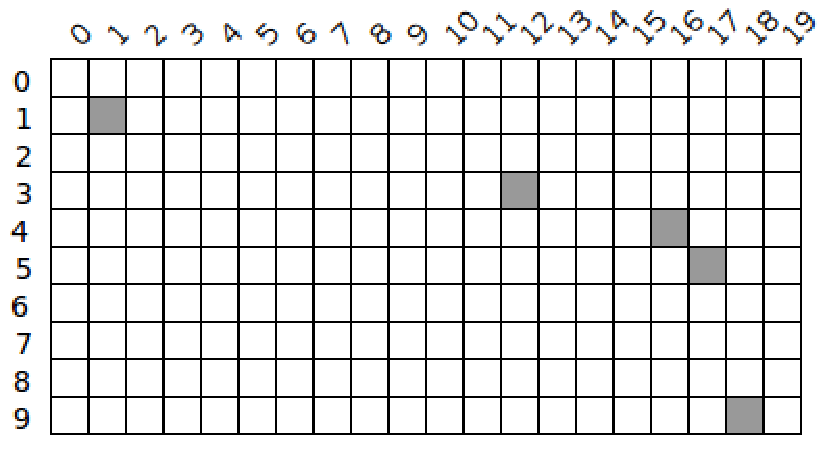
\includegraphics[scale=0.65]{Figures/PDF/Relview/XR.pdf}
		\caption{Abstraction relation $X$ for Example~\ref{ex:two_channels}.}
		\label{fig:two_channels_x}
	\end{figure}
	
	\newpage
\end{example}